\documentclass{standalone}
\usepackage{tikz}
\usetikzlibrary{patterns}
\usetikzlibrary{positioning}
\usetikzlibrary{patterns, positioning}
\usetikzlibrary{shapes.misc}
\usepackage[outline]{contour}
\contourlength{1.5pt} 
\usetikzlibrary{calc}
        \usepackage{relsize}
        \tikzset{fontscale/.style = {font=\relsize{#1}}}

\begin{document}
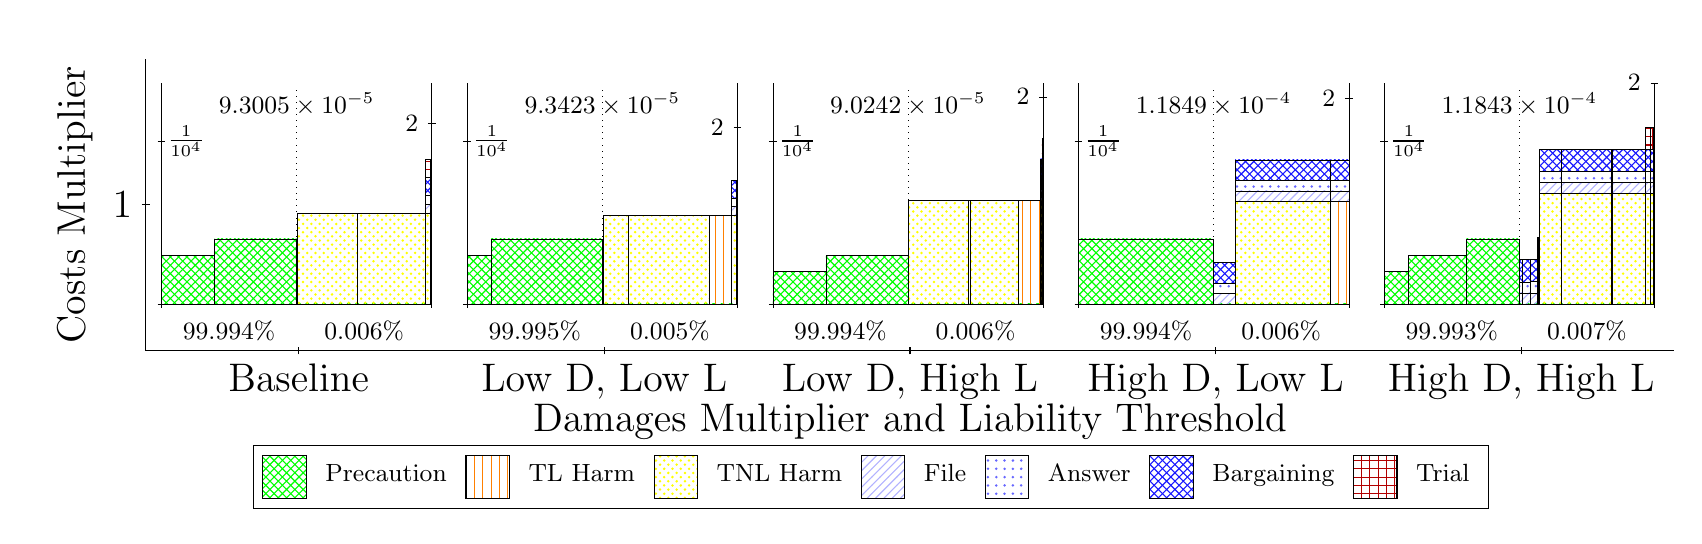
\begin{tikzpicture}
\clip(-0.5,-1.1) rectangle +(20.91,6.2);
\draw[black] (1,1) -- (1,4.7);
\node[rotate=90, fontscale=2, anchor=center] at (0.1, 2.85) {Costs Multiplier};
\draw[black] (0.95,2.85) -- (1.05,2.85);
\node[fontscale=2, anchor=east] at (0.95, 2.85) {1};

\draw[black] (1,1) -- (20.41,1);
\node[fontscale=2, anchor=center] at (10.705, 0.1) {Damages Multiplier and Liability Threshold};
\draw[black] (2.941,0.95) -- (2.941,1.05);
\node[fontscale=2, anchor=north] at (2.941, 0.95) {Baseline};
\draw[black] (6.823,0.95) -- (6.823,1.05);
\node[fontscale=2, anchor=north] at (6.823, 0.95) {Low D, Low L};
\draw[black] (10.705,0.95) -- (10.705,1.05);
\node[fontscale=2, anchor=north] at (10.705, 0.95) {Low D, High L};
\draw[black] (14.587,0.95) -- (14.587,1.05);
\node[fontscale=2, anchor=north] at (14.587, 0.95) {High D, Low L};
\draw[black] (18.469,0.95) -- (18.469,1.05);
\node[fontscale=2, anchor=north] at (18.469, 0.95) {High D, High L};


\draw[pattern=crosshatch, pattern color=green,draw=black,very thin] (1.2,1.592) rectangle (1.8725,2.2115);
\draw[pattern=crosshatch, pattern color=green,draw=black,very thin] (1.8725,1.592) rectangle (2.916,2.4181);
\draw[pattern=crosshatch, pattern color=green,draw=black,very thin] (2.916,1.592) rectangle (2.9287,1.592);
\draw[pattern=north east lines, pattern color=blue!30,draw=black,very thin] (2.916,1.592) rectangle (2.9287,1.7069);
\draw[pattern=dots,  pattern color=blue!60,draw=black,very thin] (2.916,1.7069) rectangle (2.9287,1.8217);
\draw[pattern=crosshatch,      pattern color=blue!90,draw=black,very thin] (2.916,1.8217) rectangle (2.9287,2.0514);
\draw[pattern=grid,            pattern color=red!70!black,draw=black,very thin] (2.916,2.0514) rectangle (2.9287,2.2811);
\draw[pattern=crosshatch, pattern color=green,draw=black,very thin] (2.9287,1.592) rectangle (3.6818,1.592);
\draw[pattern=crosshatch dots, pattern color=yellow,draw=black,very thin] (2.9287,1.592) rectangle (3.6818,2.7404);
\draw[pattern=crosshatch, pattern color=green,draw=black,very thin] (3.6818,1.592) rectangle (3.6897,1.592);
\draw[pattern=vertical lines, pattern color=orange,draw=black,very thin] (3.6818,1.592) rectangle (3.6897,2.7404);
\draw[pattern=crosshatch, pattern color=green,draw=black,very thin] (3.6897,1.592) rectangle (4.5556,1.592);
\draw[pattern=crosshatch dots, pattern color=yellow,draw=black,very thin] (3.6897,1.592) rectangle (4.5556,2.7404);
\draw[pattern=crosshatch, pattern color=green,draw=black,very thin] (4.5556,1.592) rectangle (4.6122,1.592);
\draw[pattern=crosshatch dots, pattern color=yellow,draw=black,very thin] (4.5556,1.592) rectangle (4.6122,2.7404);
\draw[pattern=north east lines, pattern color=blue!30,draw=black,very thin] (4.5556,2.7404) rectangle (4.6122,2.8552);
\draw[pattern=dots,  pattern color=blue!60,draw=black,very thin] (4.5556,2.8552) rectangle (4.6122,2.9701);
\draw[pattern=crosshatch,      pattern color=blue!90,draw=black,very thin] (4.5556,2.9701) rectangle (4.6122,3.1998);
\draw[pattern=grid,            pattern color=red!70!black,draw=black,very thin] (4.5556,3.1998) rectangle (4.6122,3.4294);
\draw[pattern=crosshatch, pattern color=green,draw=black,very thin] (4.6122,1.592) rectangle (4.632,1.592);
\draw[pattern=vertical lines, pattern color=orange,draw=black,very thin] (4.6122,1.592) rectangle (4.632,2.7404);
\draw[pattern=north east lines, pattern color=blue!30,draw=black,very thin] (4.6122,2.7404) rectangle (4.632,2.8552);
\draw[pattern=dots,  pattern color=blue!60,draw=black,very thin] (4.6122,2.8552) rectangle (4.632,2.9701);
\draw[pattern=crosshatch,      pattern color=blue!90,draw=black,very thin] (4.6122,2.9701) rectangle (4.632,3.1998);
\draw[pattern=grid,            pattern color=red!70!black,draw=black,very thin] (4.6122,3.1998) rectangle (4.632,3.4294);
\node[font=\small,text=black,anchor=north] at (2.916, 4.4) {$9.3005\times 10^{-5}$};
\draw[black,very thin] (1.2,1.592) -- (1.2,4.4);
\draw[black,very thin] (1.15,1.592) -- (1.25,1.592);
\node[font=\small,text=black, anchor=west] at (1.15, 1.592) {};
\draw[black,very thin] (1.15,3.6572) -- (1.25,3.6572);
\node[font=\small,text=black, anchor=west] at (1.15, 3.6572) {$\frac{1}{10^{4}}$};

\draw[black,dotted,very thin] (2.916,1.6762) -- (2.916,4.3158);
\draw[black,very thin] (4.632,1.592) -- (4.632,4.4);
\draw[black,very thin] (4.582,3.8888) -- (4.682,3.8888);
\node[font=\small,text=black, anchor=east] at (4.582, 3.8888) {\contour{white}{2}};

\draw[black,very thin] (1.2,1.592) -- (4.632,1.592);
\draw[black,very thin] (1.2,1.542) -- (1.2,1.642);
\node[font=\small,text=black, anchor=north] at (1.2, 1.542) {};
\draw[black,very thin] (4.632,1.542) -- (4.632,1.642);
\node[font=\small,text=black, anchor=north] at (4.632, 1.542) {};

\node[font=\small,text=black,anchor=south] at (2.058, 0.992) {99.994\%};
\node[font=\small,text=black,anchor=south] at (3.774, 0.992) {0.006\%};

\draw[pattern=crosshatch, pattern color=green,draw=black,very thin] (5.082,1.592) rectangle (5.3844,2.2115);
\draw[pattern=crosshatch, pattern color=green,draw=black,very thin] (5.3844,1.592) rectangle (6.798,2.4181);
\draw[pattern=crosshatch, pattern color=green,draw=black,very thin] (6.798,1.592) rectangle (6.8094,1.592);
\draw[pattern=north east lines, pattern color=blue!30,draw=black,very thin] (6.798,1.592) rectangle (6.8094,1.7043);
\draw[pattern=dots,  pattern color=blue!60,draw=black,very thin] (6.798,1.7043) rectangle (6.8094,1.8166);
\draw[pattern=crosshatch,      pattern color=blue!90,draw=black,very thin] (6.798,1.8166) rectangle (6.8094,2.0412);
\draw[pattern=crosshatch, pattern color=green,draw=black,very thin] (6.8094,1.592) rectangle (7.1215,1.592);
\draw[pattern=crosshatch dots, pattern color=yellow,draw=black,very thin] (6.8094,1.592) rectangle (7.1215,2.7149);
\draw[pattern=crosshatch, pattern color=green,draw=black,very thin] (7.1215,1.592) rectangle (7.128,1.592);
\draw[pattern=vertical lines, pattern color=orange,draw=black,very thin] (7.1215,1.592) rectangle (7.128,2.7149);
\draw[pattern=crosshatch, pattern color=green,draw=black,very thin] (7.128,1.592) rectangle (8.1612,1.592);
\draw[pattern=crosshatch dots, pattern color=yellow,draw=black,very thin] (7.128,1.592) rectangle (8.1612,2.7149);
\draw[pattern=crosshatch, pattern color=green,draw=black,very thin] (8.1612,1.592) rectangle (8.4339,1.592);
\draw[pattern=vertical lines, pattern color=orange,draw=black,very thin] (8.1612,1.592) rectangle (8.4339,2.7149);
\draw[pattern=crosshatch, pattern color=green,draw=black,very thin] (8.4339,1.592) rectangle (8.4947,1.592);
\draw[pattern=crosshatch dots, pattern color=yellow,draw=black,very thin] (8.4339,1.592) rectangle (8.4947,2.7149);
\draw[pattern=north east lines, pattern color=blue!30,draw=black,very thin] (8.4339,2.7149) rectangle (8.4947,2.8272);
\draw[pattern=dots,  pattern color=blue!60,draw=black,very thin] (8.4339,2.8272) rectangle (8.4947,2.9395);
\draw[pattern=crosshatch,      pattern color=blue!90,draw=black,very thin] (8.4339,2.9395) rectangle (8.4947,3.164);
\draw[pattern=crosshatch, pattern color=green,draw=black,very thin] (8.4947,1.592) rectangle (8.5112,1.592);
\draw[pattern=vertical lines, pattern color=orange,draw=black,very thin] (8.4947,1.592) rectangle (8.5112,2.7149);
\draw[pattern=north east lines, pattern color=blue!30,draw=black,very thin] (8.4947,2.7149) rectangle (8.5112,2.8272);
\draw[pattern=dots,  pattern color=blue!60,draw=black,very thin] (8.4947,2.8272) rectangle (8.5112,2.9395);
\draw[pattern=crosshatch,      pattern color=blue!90,draw=black,very thin] (8.4947,2.9395) rectangle (8.5112,3.164);
\draw[pattern=crosshatch, pattern color=green,draw=black,very thin] (8.5112,1.592) rectangle (8.5119,1.592);
\draw[pattern=crosshatch dots, pattern color=yellow,draw=black,very thin] (8.5112,1.592) rectangle (8.5119,2.7149);
\draw[pattern=north east lines, pattern color=blue!30,draw=black,very thin] (8.5112,2.7149) rectangle (8.5119,2.8272);
\draw[pattern=dots,  pattern color=blue!60,draw=black,very thin] (8.5112,2.8272) rectangle (8.5119,2.9395);
\draw[pattern=crosshatch,      pattern color=blue!90,draw=black,very thin] (8.5112,2.9395) rectangle (8.5119,3.164);
\draw[pattern=grid,            pattern color=red!70!black,draw=black,very thin] (8.5112,3.164) rectangle (8.5119,3.3886);
\draw[pattern=crosshatch, pattern color=green,draw=black,very thin] (8.5119,1.592) rectangle (8.514,1.592);
\draw[pattern=vertical lines, pattern color=orange,draw=black,very thin] (8.5119,1.592) rectangle (8.514,2.7149);
\draw[pattern=north east lines, pattern color=blue!30,draw=black,very thin] (8.5119,2.7149) rectangle (8.514,2.8272);
\draw[pattern=dots,  pattern color=blue!60,draw=black,very thin] (8.5119,2.8272) rectangle (8.514,2.9395);
\draw[pattern=crosshatch,      pattern color=blue!90,draw=black,very thin] (8.5119,2.9395) rectangle (8.514,3.164);
\draw[pattern=grid,            pattern color=red!70!black,draw=black,very thin] (8.5119,3.164) rectangle (8.514,3.3886);
\node[font=\small,text=black,anchor=north] at (6.798, 4.4) {$9.3423\times 10^{-5}$};
\draw[black,very thin] (5.082,1.592) -- (5.082,4.4);
\draw[black,very thin] (5.032,1.592) -- (5.132,1.592);
\node[font=\small,text=black, anchor=west] at (5.032, 1.592) {};
\draw[black,very thin] (5.032,3.6572) -- (5.132,3.6572);
\node[font=\small,text=black, anchor=west] at (5.032, 3.6572) {$\frac{1}{10^{4}}$};

\draw[black,dotted,very thin] (6.798,1.6762) -- (6.798,4.3158);
\draw[black,very thin] (8.514,1.592) -- (8.514,4.4);
\draw[black,very thin] (8.464,3.8377) -- (8.564,3.8377);
\node[font=\small,text=black, anchor=east] at (8.464, 3.8377) {\contour{white}{2}};

\draw[black,very thin] (5.082,1.592) -- (8.514,1.592);
\draw[black,very thin] (5.082,1.542) -- (5.082,1.642);
\node[font=\small,text=black, anchor=north] at (5.082, 1.542) {};
\draw[black,very thin] (8.514,1.542) -- (8.514,1.642);
\node[font=\small,text=black, anchor=north] at (8.514, 1.542) {};

\node[font=\small,text=black,anchor=south] at (5.94, 0.992) {99.995\%};
\node[font=\small,text=black,anchor=south] at (7.656, 0.992) {0.005\%};

\draw[pattern=crosshatch, pattern color=green,draw=black,very thin] (8.964,1.592) rectangle (9.6365,2.005);
\draw[pattern=crosshatch, pattern color=green,draw=black,very thin] (9.6365,1.592) rectangle (10.68,2.2115);
\draw[pattern=crosshatch, pattern color=green,draw=black,very thin] (10.68,1.592) rectangle (10.682,1.592);
\draw[pattern=north east lines, pattern color=blue!30,draw=black,very thin] (10.68,1.592) rectangle (10.682,1.7235);
\draw[pattern=dots,  pattern color=blue!60,draw=black,very thin] (10.68,1.7235) rectangle (10.682,1.8549);
\draw[pattern=crosshatch,      pattern color=blue!90,draw=black,very thin] (10.68,1.8549) rectangle (10.682,2.1178);
\draw[pattern=crosshatch, pattern color=green,draw=black,very thin] (10.682,1.592) rectangle (10.685,1.592);
\draw[pattern=north east lines, pattern color=blue!30,draw=black,very thin] (10.682,1.592) rectangle (10.685,1.7235);
\draw[pattern=dots,  pattern color=blue!60,draw=black,very thin] (10.682,1.7235) rectangle (10.685,1.8549);
\draw[pattern=crosshatch,      pattern color=blue!90,draw=black,very thin] (10.682,1.8549) rectangle (10.685,2.1178);
\draw[pattern=grid,            pattern color=red!70!black,draw=black,very thin] (10.682,2.1178) rectangle (10.685,2.3806);
\draw[pattern=crosshatch, pattern color=green,draw=black,very thin] (10.685,1.592) rectangle (11.45,1.592);
\draw[pattern=crosshatch dots, pattern color=yellow,draw=black,very thin] (10.685,1.592) rectangle (11.45,2.9064);
\draw[pattern=crosshatch, pattern color=green,draw=black,very thin] (11.45,1.592) rectangle (11.466,1.592);
\draw[pattern=vertical lines, pattern color=orange,draw=black,very thin] (11.45,1.592) rectangle (11.466,2.9064);
\draw[pattern=crosshatch, pattern color=green,draw=black,very thin] (11.466,1.592) rectangle (12.077,1.592);
\draw[pattern=crosshatch dots, pattern color=yellow,draw=black,very thin] (11.466,1.592) rectangle (12.077,2.9064);
\draw[pattern=crosshatch, pattern color=green,draw=black,very thin] (12.077,1.592) rectangle (12.364,1.592);
\draw[pattern=vertical lines, pattern color=orange,draw=black,very thin] (12.077,1.592) rectangle (12.364,2.9064);
\draw[pattern=crosshatch, pattern color=green,draw=black,very thin] (12.364,1.592) rectangle (12.376,1.592);
\draw[pattern=crosshatch dots, pattern color=yellow,draw=black,very thin] (12.364,1.592) rectangle (12.376,2.9064);
\draw[pattern=north east lines, pattern color=blue!30,draw=black,very thin] (12.364,2.9064) rectangle (12.376,3.0378);
\draw[pattern=dots,  pattern color=blue!60,draw=black,very thin] (12.364,3.0378) rectangle (12.376,3.1693);
\draw[pattern=crosshatch,      pattern color=blue!90,draw=black,very thin] (12.364,3.1693) rectangle (12.376,3.4321);
\draw[pattern=crosshatch, pattern color=green,draw=black,very thin] (12.376,1.592) rectangle (12.379,1.592);
\draw[pattern=vertical lines, pattern color=orange,draw=black,very thin] (12.376,1.592) rectangle (12.379,2.9064);
\draw[pattern=north east lines, pattern color=blue!30,draw=black,very thin] (12.376,2.9064) rectangle (12.379,3.0378);
\draw[pattern=dots,  pattern color=blue!60,draw=black,very thin] (12.376,3.0378) rectangle (12.379,3.1693);
\draw[pattern=crosshatch,      pattern color=blue!90,draw=black,very thin] (12.376,3.1693) rectangle (12.379,3.4321);
\draw[pattern=crosshatch, pattern color=green,draw=black,very thin] (12.379,1.592) rectangle (12.388,1.592);
\draw[pattern=crosshatch dots, pattern color=yellow,draw=black,very thin] (12.379,1.592) rectangle (12.388,2.9064);
\draw[pattern=north east lines, pattern color=blue!30,draw=black,very thin] (12.379,2.9064) rectangle (12.388,3.0378);
\draw[pattern=dots,  pattern color=blue!60,draw=black,very thin] (12.379,3.0378) rectangle (12.388,3.1693);
\draw[pattern=crosshatch,      pattern color=blue!90,draw=black,very thin] (12.379,3.1693) rectangle (12.388,3.4321);
\draw[pattern=grid,            pattern color=red!70!black,draw=black,very thin] (12.379,3.4321) rectangle (12.388,3.695);
\draw[pattern=crosshatch, pattern color=green,draw=black,very thin] (12.388,1.592) rectangle (12.396,1.592);
\draw[pattern=vertical lines, pattern color=orange,draw=black,very thin] (12.388,1.592) rectangle (12.396,2.9064);
\draw[pattern=north east lines, pattern color=blue!30,draw=black,very thin] (12.388,2.9064) rectangle (12.396,3.0378);
\draw[pattern=dots,  pattern color=blue!60,draw=black,very thin] (12.388,3.0378) rectangle (12.396,3.1693);
\draw[pattern=crosshatch,      pattern color=blue!90,draw=black,very thin] (12.388,3.1693) rectangle (12.396,3.4321);
\draw[pattern=grid,            pattern color=red!70!black,draw=black,very thin] (12.388,3.4321) rectangle (12.396,3.695);
\node[font=\small,text=black,anchor=north] at (10.68, 4.4) {$9.0242\times 10^{-5}$};
\draw[black,very thin] (8.964,1.592) -- (8.964,4.4);
\draw[black,very thin] (8.914,1.592) -- (9.014,1.592);
\node[font=\small,text=black, anchor=west] at (8.914, 1.592) {};
\draw[black,very thin] (8.914,3.6571) -- (9.014,3.6571);
\node[font=\small,text=black, anchor=west] at (8.914, 3.6571) {$\frac{1}{10^{4}}$};

\draw[black,dotted,very thin] (10.68,1.6762) -- (10.68,4.3158);
\draw[black,very thin] (12.396,1.592) -- (12.396,4.4);
\draw[black,very thin] (12.346,4.2207) -- (12.446,4.2207);
\node[font=\small,text=black, anchor=east] at (12.346, 4.2207) {\contour{white}{2}};

\draw[black,very thin] (8.964,1.592) -- (12.396,1.592);
\draw[black,very thin] (8.964,1.542) -- (8.964,1.642);
\node[font=\small,text=black, anchor=north] at (8.964, 1.542) {};
\draw[black,very thin] (12.396,1.542) -- (12.396,1.642);
\node[font=\small,text=black, anchor=north] at (12.396, 1.542) {};

\node[font=\small,text=black,anchor=south] at (9.822, 0.992) {99.994\%};
\node[font=\small,text=black,anchor=south] at (11.538, 0.992) {0.006\%};

\draw[pattern=crosshatch, pattern color=green,draw=black,very thin] (12.846,1.592) rectangle (14.562,2.4181);
\draw[pattern=crosshatch, pattern color=green,draw=black,very thin] (14.562,1.592) rectangle (14.833,1.5921);
\draw[pattern=north east lines, pattern color=blue!30,draw=black,very thin] (14.562,1.5921) rectangle (14.833,1.7226);
\draw[pattern=dots,  pattern color=blue!60,draw=black,very thin] (14.562,1.7226) rectangle (14.833,1.8531);
\draw[pattern=crosshatch,      pattern color=blue!90,draw=black,very thin] (14.562,1.8531) rectangle (14.833,2.1142);
\draw[pattern=crosshatch, pattern color=green,draw=black,very thin] (14.833,1.592) rectangle (16.043,1.5921);
\draw[pattern=crosshatch dots, pattern color=yellow,draw=black,very thin] (14.833,1.5921) rectangle (16.043,2.8974);
\draw[pattern=north east lines, pattern color=blue!30,draw=black,very thin] (14.833,2.8974) rectangle (16.043,3.0279);
\draw[pattern=dots,  pattern color=blue!60,draw=black,very thin] (14.833,3.0279) rectangle (16.043,3.1585);
\draw[pattern=crosshatch,      pattern color=blue!90,draw=black,very thin] (14.833,3.1585) rectangle (16.043,3.4196);
\draw[pattern=crosshatch, pattern color=green,draw=black,very thin] (16.043,1.592) rectangle (16.278,1.5921);
\draw[pattern=vertical lines, pattern color=orange,draw=black,very thin] (16.043,1.5921) rectangle (16.278,2.8974);
\draw[pattern=north east lines, pattern color=blue!30,draw=black,very thin] (16.043,2.8974) rectangle (16.278,3.0279);
\draw[pattern=dots,  pattern color=blue!60,draw=black,very thin] (16.043,3.0279) rectangle (16.278,3.1585);
\draw[pattern=crosshatch,      pattern color=blue!90,draw=black,very thin] (16.043,3.1585) rectangle (16.278,3.4196);
\node[font=\small,text=black,anchor=north] at (14.562, 4.4) {$1.1849\times 10^{-4}$};
\draw[black,very thin] (12.846,1.592) -- (12.846,4.4);
\draw[black,very thin] (12.796,1.592) -- (12.896,1.592);
\node[font=\small,text=black, anchor=west] at (12.796, 1.592) {};
\draw[black,very thin] (12.796,3.6571) -- (12.896,3.6571);
\node[font=\small,text=black, anchor=west] at (12.796, 3.6571) {$\frac{1}{10^{4}}$};

\draw[black,dotted,very thin] (14.562,1.6762) -- (14.562,4.3158);
\draw[black,very thin] (16.278,1.592) -- (16.278,4.4);
\draw[black,very thin] (16.228,4.2027) -- (16.328,4.2027);
\node[font=\small,text=black, anchor=east] at (16.228, 4.2027) {\contour{white}{2}};

\draw[black,very thin] (12.846,1.592) -- (16.278,1.592);
\draw[black,very thin] (12.846,1.542) -- (12.846,1.642);
\node[font=\small,text=black, anchor=north] at (12.846, 1.542) {};
\draw[black,very thin] (16.278,1.542) -- (16.278,1.642);
\node[font=\small,text=black, anchor=north] at (16.278, 1.542) {};

\node[font=\small,text=black,anchor=south] at (13.704, 0.992) {99.994\%};
\node[font=\small,text=black,anchor=south] at (15.42, 0.992) {0.006\%};

\draw[pattern=crosshatch, pattern color=green,draw=black,very thin] (16.728,1.592) rectangle (17.03,2.005);
\draw[pattern=crosshatch, pattern color=green,draw=black,very thin] (17.03,1.592) rectangle (17.772,2.2115);
\draw[pattern=crosshatch, pattern color=green,draw=black,very thin] (17.772,1.592) rectangle (18.444,2.4181);
\draw[pattern=crosshatch, pattern color=green,draw=black,very thin] (18.444,1.592) rectangle (18.479,1.592);
\draw[pattern=north east lines, pattern color=blue!30,draw=black,very thin] (18.444,1.592) rectangle (18.479,1.7324);
\draw[pattern=dots,  pattern color=blue!60,draw=black,very thin] (18.444,1.7324) rectangle (18.479,1.8728);
\draw[pattern=crosshatch,      pattern color=blue!90,draw=black,very thin] (18.444,1.8728) rectangle (18.479,2.1536);
\draw[pattern=crosshatch, pattern color=green,draw=black,very thin] (18.479,1.592) rectangle (18.579,1.592);
\draw[pattern=north east lines, pattern color=blue!30,draw=black,very thin] (18.479,1.592) rectangle (18.579,1.7324);
\draw[pattern=dots,  pattern color=blue!60,draw=black,very thin] (18.479,1.7324) rectangle (18.579,1.8728);
\draw[pattern=crosshatch,      pattern color=blue!90,draw=black,very thin] (18.479,1.8728) rectangle (18.579,2.1536);
\draw[pattern=crosshatch, pattern color=green,draw=black,very thin] (18.579,1.592) rectangle (18.678,1.5921);
\draw[pattern=north east lines, pattern color=blue!30,draw=black,very thin] (18.579,1.5921) rectangle (18.678,1.7325);
\draw[pattern=dots,  pattern color=blue!60,draw=black,very thin] (18.579,1.7325) rectangle (18.678,1.8729);
\draw[pattern=crosshatch,      pattern color=blue!90,draw=black,very thin] (18.579,1.8729) rectangle (18.678,2.1536);
\draw[pattern=crosshatch, pattern color=green,draw=black,very thin] (18.678,1.592) rectangle (18.687,1.592);
\draw[pattern=north east lines, pattern color=blue!30,draw=black,very thin] (18.678,1.592) rectangle (18.687,1.7324);
\draw[pattern=dots,  pattern color=blue!60,draw=black,very thin] (18.678,1.7324) rectangle (18.687,1.8728);
\draw[pattern=crosshatch,      pattern color=blue!90,draw=black,very thin] (18.678,1.8728) rectangle (18.687,2.1536);
\draw[pattern=grid,            pattern color=red!70!black,draw=black,very thin] (18.678,2.1536) rectangle (18.687,2.4344);
\draw[pattern=crosshatch, pattern color=green,draw=black,very thin] (18.687,1.592) rectangle (18.696,1.592);
\draw[pattern=north east lines, pattern color=blue!30,draw=black,very thin] (18.687,1.592) rectangle (18.696,1.7324);
\draw[pattern=dots,  pattern color=blue!60,draw=black,very thin] (18.687,1.7324) rectangle (18.696,1.8728);
\draw[pattern=crosshatch,      pattern color=blue!90,draw=black,very thin] (18.687,1.8728) rectangle (18.696,2.1536);
\draw[pattern=grid,            pattern color=red!70!black,draw=black,very thin] (18.687,2.1536) rectangle (18.696,2.4344);
\draw[pattern=crosshatch, pattern color=green,draw=black,very thin] (18.696,1.592) rectangle (18.975,1.592);
\draw[pattern=crosshatch dots, pattern color=yellow,draw=black,very thin] (18.696,1.592) rectangle (18.975,2.996);
\draw[pattern=north east lines, pattern color=blue!30,draw=black,very thin] (18.696,2.996) rectangle (18.975,3.1364);
\draw[pattern=dots,  pattern color=blue!60,draw=black,very thin] (18.696,3.1364) rectangle (18.975,3.2768);
\draw[pattern=crosshatch,      pattern color=blue!90,draw=black,very thin] (18.696,3.2768) rectangle (18.975,3.5576);
\draw[pattern=crosshatch, pattern color=green,draw=black,very thin] (18.975,1.592) rectangle (19.609,1.592);
\draw[pattern=crosshatch dots, pattern color=yellow,draw=black,very thin] (18.975,1.592) rectangle (19.609,2.996);
\draw[pattern=north east lines, pattern color=blue!30,draw=black,very thin] (18.975,2.996) rectangle (19.609,3.1364);
\draw[pattern=dots,  pattern color=blue!60,draw=black,very thin] (18.975,3.1364) rectangle (19.609,3.2768);
\draw[pattern=crosshatch,      pattern color=blue!90,draw=black,very thin] (18.975,3.2768) rectangle (19.609,3.5576);
\draw[pattern=crosshatch, pattern color=green,draw=black,very thin] (19.609,1.592) rectangle (19.621,1.592);
\draw[pattern=vertical lines, pattern color=orange,draw=black,very thin] (19.609,1.592) rectangle (19.621,2.996);
\draw[pattern=north east lines, pattern color=blue!30,draw=black,very thin] (19.609,2.996) rectangle (19.621,3.1364);
\draw[pattern=dots,  pattern color=blue!60,draw=black,very thin] (19.609,3.1364) rectangle (19.621,3.2768);
\draw[pattern=crosshatch,      pattern color=blue!90,draw=black,very thin] (19.609,3.2768) rectangle (19.621,3.5576);
\draw[pattern=crosshatch, pattern color=green,draw=black,very thin] (19.621,1.592) rectangle (20.04,1.5921);
\draw[pattern=crosshatch dots, pattern color=yellow,draw=black,very thin] (19.621,1.5921) rectangle (20.04,2.996);
\draw[pattern=north east lines, pattern color=blue!30,draw=black,very thin] (19.621,2.996) rectangle (20.04,3.1364);
\draw[pattern=dots,  pattern color=blue!60,draw=black,very thin] (19.621,3.1364) rectangle (20.04,3.2768);
\draw[pattern=crosshatch,      pattern color=blue!90,draw=black,very thin] (19.621,3.2768) rectangle (20.04,3.5576);
\draw[pattern=crosshatch, pattern color=green,draw=black,very thin] (20.04,1.592) rectangle (20.11,1.592);
\draw[pattern=crosshatch dots, pattern color=yellow,draw=black,very thin] (20.04,1.592) rectangle (20.11,2.996);
\draw[pattern=north east lines, pattern color=blue!30,draw=black,very thin] (20.04,2.996) rectangle (20.11,3.1364);
\draw[pattern=dots,  pattern color=blue!60,draw=black,very thin] (20.04,3.1364) rectangle (20.11,3.2768);
\draw[pattern=crosshatch,      pattern color=blue!90,draw=black,very thin] (20.04,3.2768) rectangle (20.11,3.5576);
\draw[pattern=grid,            pattern color=red!70!black,draw=black,very thin] (20.04,3.5576) rectangle (20.11,3.8384);
\draw[pattern=crosshatch, pattern color=green,draw=black,very thin] (20.11,1.592) rectangle (20.112,1.592);
\draw[pattern=vertical lines, pattern color=orange,draw=black,very thin] (20.11,1.592) rectangle (20.112,2.996);
\draw[pattern=north east lines, pattern color=blue!30,draw=black,very thin] (20.11,2.996) rectangle (20.112,3.1364);
\draw[pattern=dots,  pattern color=blue!60,draw=black,very thin] (20.11,3.1364) rectangle (20.112,3.2768);
\draw[pattern=crosshatch,      pattern color=blue!90,draw=black,very thin] (20.11,3.2768) rectangle (20.112,3.5576);
\draw[pattern=grid,            pattern color=red!70!black,draw=black,very thin] (20.11,3.5576) rectangle (20.112,3.8384);
\draw[pattern=crosshatch, pattern color=green,draw=black,very thin] (20.112,1.592) rectangle (20.144,1.592);
\draw[pattern=crosshatch dots, pattern color=yellow,draw=black,very thin] (20.112,1.592) rectangle (20.144,2.996);
\draw[pattern=north east lines, pattern color=blue!30,draw=black,very thin] (20.112,2.996) rectangle (20.144,3.1364);
\draw[pattern=dots,  pattern color=blue!60,draw=black,very thin] (20.112,3.1364) rectangle (20.144,3.2768);
\draw[pattern=crosshatch,      pattern color=blue!90,draw=black,very thin] (20.112,3.2768) rectangle (20.144,3.5576);
\draw[pattern=grid,            pattern color=red!70!black,draw=black,very thin] (20.112,3.5576) rectangle (20.144,3.8384);
\draw[pattern=crosshatch, pattern color=green,draw=black,very thin] (20.144,1.592) rectangle (20.16,1.592);
\draw[pattern=vertical lines, pattern color=orange,draw=black,very thin] (20.144,1.592) rectangle (20.16,2.996);
\draw[pattern=north east lines, pattern color=blue!30,draw=black,very thin] (20.144,2.996) rectangle (20.16,3.1364);
\draw[pattern=dots,  pattern color=blue!60,draw=black,very thin] (20.144,3.1364) rectangle (20.16,3.2768);
\draw[pattern=crosshatch,      pattern color=blue!90,draw=black,very thin] (20.144,3.2768) rectangle (20.16,3.5576);
\draw[pattern=grid,            pattern color=red!70!black,draw=black,very thin] (20.144,3.5576) rectangle (20.16,3.8384);
\node[font=\small,text=black,anchor=north] at (18.444, 4.4) {$1.1843\times 10^{-4}$};
\draw[black,very thin] (16.728,1.592) -- (16.728,4.4);
\draw[black,very thin] (16.678,1.592) -- (16.778,1.592);
\node[font=\small,text=black, anchor=west] at (16.678, 1.592) {};
\draw[black,very thin] (16.678,3.6571) -- (16.778,3.6571);
\node[font=\small,text=black, anchor=west] at (16.678, 3.6571) {$\frac{1}{10^{4}}$};

\draw[black,dotted,very thin] (18.444,1.6762) -- (18.444,4.3158);
\draw[black,very thin] (20.16,1.592) -- (20.16,4.4);
\draw[black,very thin] (20.11,4.3999) -- (20.21,4.3999);
\node[font=\small,text=black, anchor=east] at (20.11, 4.3999) {\contour{white}{2}};

\draw[black,very thin] (16.728,1.592) -- (20.16,1.592);
\draw[black,very thin] (16.728,1.542) -- (16.728,1.642);
\node[font=\small,text=black, anchor=north] at (16.728, 1.542) {};
\draw[black,very thin] (20.16,1.542) -- (20.16,1.642);
\node[font=\small,text=black, anchor=north] at (20.16, 1.542) {};

\node[font=\small,text=black,anchor=south] at (17.586, 0.992) {99.993\%};
\node[font=\small,text=black,anchor=south] at (19.302, 0.992) {0.007\%};

\coordinate (LegendAnchor) at (10.205000000000002,0);
\begin{scope}[align=center]
\matrix[scale=0.6,draw=black,below=0.2cm of LegendAnchor,nodes={draw},column sep=0.12cm]{
\node[rectangle,draw,minimum width=0.55cm,minimum height=0.55cm,pattern=crosshatch, pattern color=green]{}; &
        \node[draw=none,font=\small]{Precaution}; &
\node[rectangle,draw,minimum width=0.55cm,minimum height=0.55cm,pattern=vertical lines, pattern color=orange]{}; &
        \node[draw=none,font=\small]{TL Harm}; &
\node[rectangle,draw,minimum width=0.55cm,minimum height=0.55cm,pattern=crosshatch dots, pattern color=yellow]{}; &
        \node[draw=none,font=\small]{TNL Harm}; &
\node[rectangle,draw,minimum width=0.55cm,minimum height=0.55cm,pattern=north east lines, pattern color=blue!30]{}; &
        \node[draw=none,font=\small]{File}; &
\node[rectangle,draw,minimum width=0.55cm,minimum height=0.55cm,pattern=dots, pattern color=blue!60]{}; &
        \node[draw=none,font=\small]{Answer}; &
\node[rectangle,draw,minimum width=0.55cm,minimum height=0.55cm,pattern=crosshatch, pattern color=blue!90]{}; &
        \node[draw=none,font=\small]{Bargaining}; &
\node[rectangle,draw,minimum width=0.55cm,minimum height=0.55cm,pattern=grid, pattern color=red!70!black]{}; &
        \node[draw=none,font=\small]{Trial}; \\
};\end{scope}

\end{tikzpicture}
\end{document}